\section{A simple case} \label{section:simple-case}

Using different models for slight variations of the same problem is quite commonplace in the industry. For instance, UberEats has a vast, hierarchical set of models for every country, region, and city for calculating the estimated time of delivery \cite{li2017scaling}. We have also found, that in order to best process an academic publication, knowing its domain is essential. The reason for this can be (among others) the wildly different vocabularies of different domains. For example, the term \textit{framework} in computer science almost always refers to a software artifact (usually implying high tech-transfer potential), while in every other domain, \textit{framework} is used to describe theoretical models that are less central to practical applications. Of course, it is not merely the meaning of the terms but more importantly, their distribution that varies significantly. Therefore, the topic of this section is to design and develop a domain prediction model for academic papers.

\subsection{Background}

Fortunately, this is one of the oldest subjects of text classification. In fact, Maron introduced the Naive Bayes classifier in 1961 for exactly this purpose: classifying documents' subjects. To look at a more recent approach, SciBERT \cite{beltagy2019scibert} --- a BERT \cite{devlin2018bert} model pretrained on academic publications --- was also used for a similar task in which the domains of sentences have to be decided\footnote{\href{https://paperswithcode.com/sota/sentence-classification-on-paper-field}{paperswithcode.com/sota/sentence-classification-on-paper-field}}. It achieved an F1-score of $0.6571$ after being pretrained on the Semantic Scholar Corpus (SSC) \cite{Lo2020S2ORCTS} and finetuned on the train split of the Microsoft Academic Graph (MAG) dataset \cite{wang2019review}\footnote{SciBERT was applied to a preprocessed version of this dataset available at \href{https://github.com/allenai/scibert/tree/master/data/text_classification/mag}{github.com/allenai/scibert/tree/master/data/text\_classification/mag}}.

\begin{displayquote}
\textbf{Design note} After getting familiar with the context, it is time to focus on experimenting and developing our domain prediction service. At the same time, the difficulties encountered should be noted and integrated into GreatAI's design.
\end{displayquote}

\subsection{Data}

Two datasets will be considered for the experiments. SciBERT's MAG and the SSC. The former is used to compare the results with SciBERT's, while the latter is utilised for training a model for production purposes because it has 19 labels compared with MAG's 7 and it also contains abstracts instead of just sentences, thus, it is more fitting for our use-case.

SciBERT's version of the MAG dataset has 84 thousand and 22.3 thousand sentences in its train and test splits respectively. These are mostly in English and have all punctuation and casing removed. Each sentence is classified as belonging to one of seven fields. Figure \ref{fig:mag-distribtion} shows that the classes have a uniform distribution. 

\begin{figure}
    \centering
    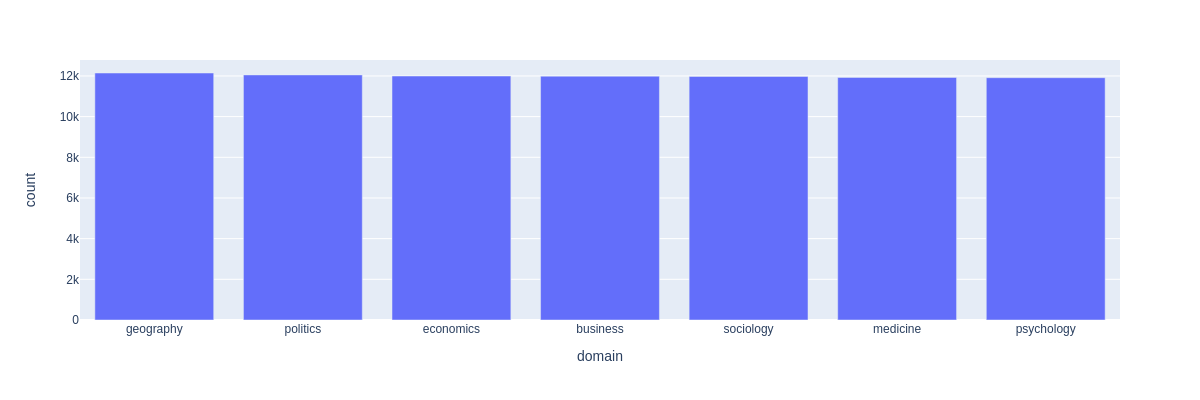
\includegraphics[width=\linewidth]{figures/mag-distribution.png}
    \caption{Class distribution of the MAG  \cite{wang2019review} dataset's 84000 sentences in its \textit{train} split.}
    \label{fig:mag-distribtion}
\end{figure}

SSC is much larger: it contains over 80 million abstracts. Having more data certainly helps in sampling the term distribution more accurately, the law of diminishing returns apply, especially when using simple models. Therefore, the data will be randomly downsampled to leave us with a more manageable couple of hundred megabytes of abstracts. We can see the distribution of class labels in Figure \ref{fig:ss-distribution}. The dataset is considerably less balanced: \textit{medicine} is by far the most popular field.

\begin{figure}
    \centering
    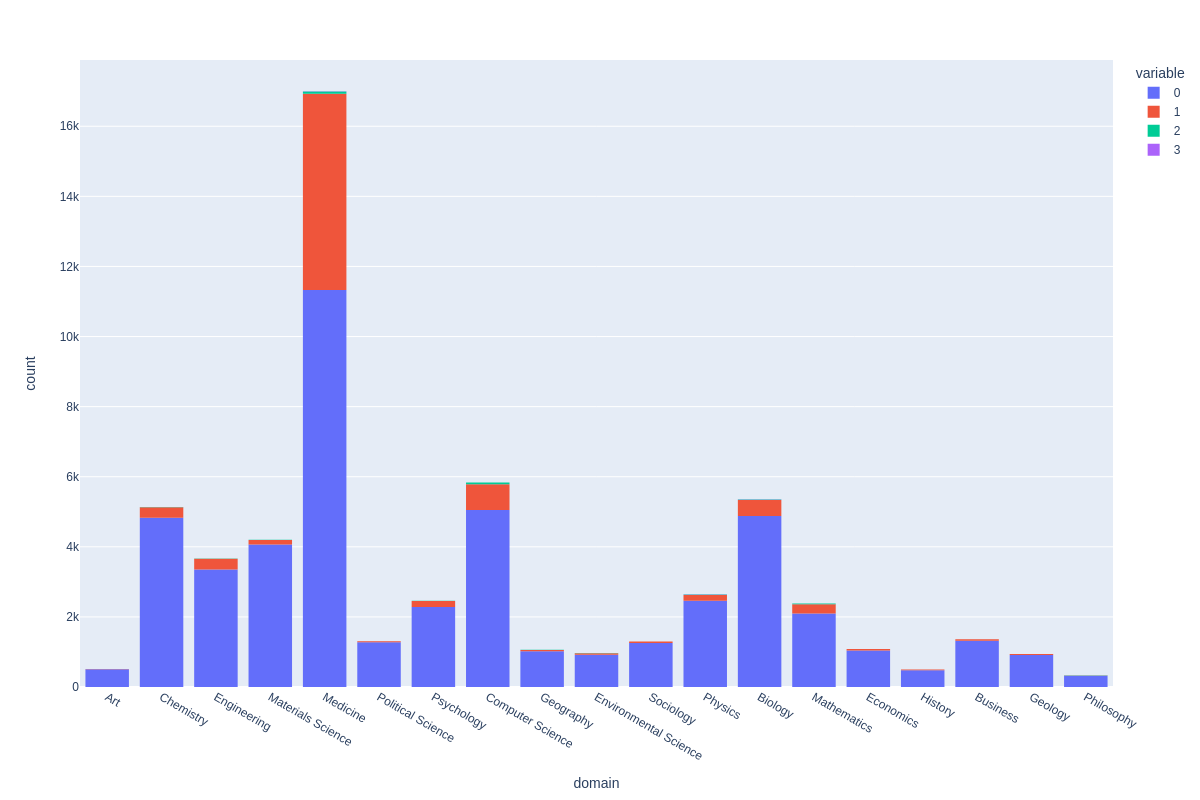
\includegraphics[width=\linewidth]{figures/ss-distribution.png}
    \caption{Label distribution of the Semantic Scholar dataset \cite{Lo2020S2ORCTS}. The \textit{variable} refers to the position of the domain in the list of domains assigned to a paper.}
    \label{fig:ss-distribution}
\end{figure}

\begin{displayquote}
\textbf{Where should we store this data?} "On my machine" seems like an easy answer. However, if we have a team working with the data or it has intrinsic value, it must be stored in an easy-to-access, potentially redundant way. Serban et al. \cite{serban2020adoption} expressed this need in the following best practice: \textit{Make Data Sets Available on Shared Infrastructure (private or public)}. Meanwhile, wherever data is stored, it should also be versioned to satisfy the next best practice: \textit{Use Versioning for Data, Model, Configurations and Training Scripts}.
\end{displayquote}

MAG needs no further preprocessing if we aim to match SciBERT's setup \cite{beltagy2019scibert}. But since SSC contains a heap of metadata, the relevant parts have to be extracted and preprocessed. In this case, these are the the concatenation of the abstract's text, paper's title and the journal's name along with the paper's domains (there can be multiple domains for a single paper, it is a mulitlabel classification task). Lastly, the non-English entries are discarded because we only expect to process papers in  English.

\begin{displayquote}
\textbf{How should we preprocess the data?} These simple processing steps (filter, map, project) are almost always present in the data science life-cycle. For example, cleaning the input text from various HTML, OCR, PDF, or \LaTeX \hskip 0.12cm extraction artifacts is almost always necessary for text analysis. This is captured in the AI best-practices collection under the following category: \textit{Write Reusable Scripts for Data Cleaning and Merging}. Also, the best practice of \textit{Test all Feature Extraction Code} is somewhat applicable: the applied processing steps must not introduce unwanted artifacts.
\end{displayquote}

\subsection{Methods}

Since the aim is to classify papers to allow the ScoutinScience platform to select models which have been trained on a matching vocabulary (and domain), it seems reasonable that only considering the distribution (frequencies) of individual terms may be sufficient. To test this hypothesis, a unigram language model (Multinomial Naive Bayes) is constructed and its accuracy is compared with SciBERT's. The former definitely aligns with the advice to \textit{Use The Most Efficient Models}.

Using the MNB implementation of scikit-learn \cite{pedregosa2011scikit}, it only took a couple of lines to create, hyperparameter-optimise, and test a text classifier. Including data loading and visualisations, it takes 71 LOC to be more precise. \footnote{The code is available at \href{https://github.com/ScoutinScience/great-ai/blob/main/examples/simple-mag/train.ipynb}{github.com/ScoutinScience/great-ai/blob/main/examples/simple-mag/train.ipynb}} This further proves relatively how simple it is to apply existing algorithms. The code can be considered for satisfying the \textit{Automate Hyper-Parameter Optimisation} best-practice, since it also implements an automated hyperparameter sweep. 

The sentences are tokenised into words and vectorised with TF-IDF (with logarithmic term frequency) \cite{buckley1985implementation}, the hyperparameters found via 3-fold cross-validation on the \textit{train} split lead to filtering out tokens which occur in fewer than 5 documents or more than 5\% of the documents.

\begin{displayquote}
\textbf{What could be automated here?} As discussed in Section \ref{section:accessible-ai}, libraries exposing algorithms and state-of-the-art models can already be considered mature and accessible. In this case, only scikit-learn was utilised, but subjectively, most popular libraries have a similarly easy to use use API. Therefore, I see no urgent need for further action regarding the \textit{experimentation} step of the life-cycle in connection with the AI best practices.
\end{displayquote}

\subsection{Results \& Discussion}

\begin{figure}
    \centering
    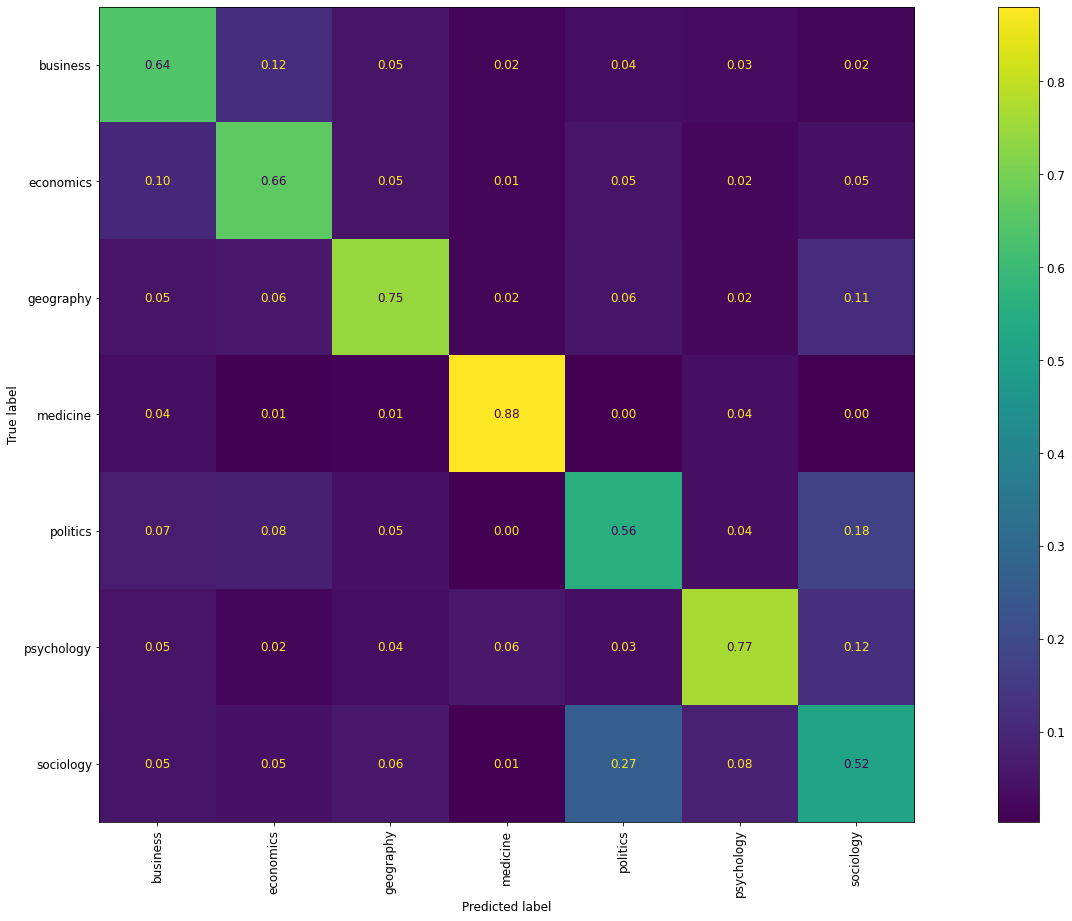
\includegraphics[width=0.8\linewidth]{figures/confusion-matrix.png}
    \caption{Confusion matrix of a Naive Bayes classifier on the MAG dataset's sentences. The matrix is normalised column-wise. Notice, how most mistakes happen between semantically similar classes, for instance: \textit{politics} -- \textit{sociology} or \textit{business} -- \textit{economics}.}
    \label{fig:mag-confusion}
\end{figure}

\begin{figure}
    \centering
    \includegraphics[width=\linewidth]{figures/ss-confusion.png}
    \caption{Confusion matrix of a Naive Bayes classifier on the SSC dataset's sentences. The matrix is normalised column-wise. Notice, how most mistakes happen between semantically similar classes, for instance:  \textit{philosohpy} -- \textit{sociology} or \textit{history} -- \textit{art}.}
    \label{fig:ss-confusion}
\end{figure}

When this model is applied to the \textit{test} split of MAG, we get the confusion matrix of Figure \ref{fig:mag-confusion}. This Naive Bayes classifier achieves a whopping $0.6795$ F1-score. This is $3.4\%$ better than SciBERT's on the same dataset. Thus, it seems, MNB clearly outperforms SciBERT for this particular use-case: it is not only more accurate, its model is magnitudes smaller, while it is also considerably faster to train (or finetune in the case of SciBERT) and use.

It is, of course, not entirely surprising that the sophisticated transformer architecture of SciBERT is not necessary for a plain task like this. Apart from phrases, the relation between separate words of a sentence do not carry nearly as much discriminative power as the identity of the terms\footnote{On a similar note, the independence assumption of Naive Bayes is often less wrong than it might seem \cite{hand2001idiot}.}, hence there is little reason for using an attention mechanism. The fact that SciBERT even works in any way on this task is already a testament to its general applicability. Nevertheless, this short experiment has proved that we can safely opt for using MNB for production.

Since Multinomial Naive Bayes is best at returning a single label and SSC is has multiple labels per datapoint: for evaluation purposes, it is checked whether the returned label is contained in the labels of the ground truth. On this dataset, MNB achieves a significantly lower macro-average F1-score which is 0.49. The weighted-average F1 is 0.61 and the overall accuracy is 62\%. The large difference between the macro and weighted averages come from the unbalanced distribution of the labels, better performance could be achieved by uniformly sampling from each class.

The lower F1-score is not surprising because there are more than twice as many classes in this dataset,  Additionally, the mistakes made are defendable when we look at Figure \ref{fig:ss-confusion}: most of them are between close or related classes.

\begin{displayquote}
This is the usual point where papers conclude: a proof-of-concept/prototype has been built and its performance demonstrated, measured --- and usually --- explained. Nonetheless, in an industrial setting, our problem is far from being solved: it has yet to be deployed.
\end{displayquote}

\subsection{Deployment}

First, an inference function needs to be written that can take an input on the fly and calculate a corresponding prediction. Since we aim to follow the best practices, namely: \textit{Explain Results and Decisions to Users} and \textit{Employ Interpretable Models When Possible}, giving an explanation of the results is expected. Fortunately, with our simple model it's easy to determine the most influential weights, thus, words. The last deployment step may be to provide access to our model for others.

\begin{displayquote}
\textbf{How do we provide an interface for the inference function?} We either have an offline or online inference workflow (or both). For the former, we have to provide a way to use it in batch processing; a simple Python function may be adequate for this purpose, though, allowing it to be easily (or automatically) parallelised would make its consumers' DX better. If it is an online-workflow, we must have a service running continuously and accepting input at any time. This can be achieved by a remote procedure call (RPC) interface, or more commonly, a web API. Developers usually refer to these as REST API-s, sometimes, they even follow the conventions of REST. Either ways, we must develop a wrapper over the service in order to make it available for other internal/external consumers.
\end{displayquote}

According to the research on the adoption of best practices, this is where many real-world projects conclude. This happens to be \textbf{the gap}. Believing that solely focusing on the research and experiments is good enough is a fallacy: when following this approach, the deployment step ends up being a rushed attempt of wrapping the \textit{AI} and putting it in the production environment. This is inarguably a deployment. However, it follows very few of the best practices. This can lead to suboptimal real-life performance, lack of accountability, lack of opportunity to improve, and can overall lead to negative societal impact \cite{o2016weapons}.

\begin{displayquote}
\textbf{How could we implement more best practices?} The most notable missing best practices are the lack of automated deployment, automated regression testing, online monitoring, persisting the traces, graceful error-handling, taking feedback on the results (if possible in the use-case), calculating the online accuracy based on the feedback, and retraining the model if necessary using novel data. These all correspond to a best practice.
\end{displayquote}
